\documentclass[a4paper,14pt]{article}
\usepackage[left=2cm,right=2cm, top=2cm,bottom=2cm, bindingoffset=0cm]{geometry}

\usepackage[T2A]{fontenc}
\usepackage[utf8]{inputenc}
\usepackage[english,russian]{babel}

\usepackage{amsmath,amsfonts,amssymb,amsthm,mathtools, graphicx}

\usepackage{fancybox,fancyhdr}

\usepackage{tabularx}
\usepackage{multirow}
\usepackage{bigstrut}
\usepackage{booktabs}
\usepackage{float}
\graphicspath{{pictures/}}
\DeclareGraphicsExtensions{.pdf,.png,.jpg}
\documentclass{article}
\usepackage{xcolor}

% \pagecolor{gray}  % фон всей страницы
% \color{white}      % цвет текста

\author{Ануфриев Андрей}
\title{Отчет по лабораторной работе № \\}
\date{\today}


\begin{document}

    \begin{figure}[h]
        \centering
        \begin{minipage}{0.45\linewidth}
            \centering
            
\includegraphics[width=\linewidth]{slogan_chernyy.png}
            \label{fig:slogan}
        \end{minipage}
        \hfill
        \begin{minipage}{0.45\linewidth}
            \centering
            
\includegraphics[width=\linewidth]{itmo-cs-logo.png}
            \label{fig:logo}
        \end{minipage}
    \end{figure}
    \begin{table}[htbp]
        \centering
        \begin{tabular}{lrlr}
            Группа & \qquad \qquad P3219 & К работе допущен & \qquad \qquad \qquad \qquad \qquad \qquad \\
            \cmidrule{2-2}\cmidrule{4-4}
            Студент &  \qquad \qquad Ануфриев Андрей  & Работа выполнена & \qquad \qquad \qquad \qquad \qquad \qquad \\
            \cmidrule{2-2}\cmidrule{4-4}
            Преподаватель & \qquad \qquad Коробков М.П. & Отчет принят & \qquad \qquad \qquad \qquad \qquad \qquad \\
            \cmidrule{2-2}\cmidrule{4-4}
        \end{tabular}%
    \end{table}%
    \vspace{2cm}
    \begin{center}
        \LARGE
        Отчет по лабораторной работе № 1.09 \\
        Определение момента инерции методом крутильных колебаний

    \end{center}
    \vspace{13cm}
    \begin{center}
        2025 год
    \end{center}
    \newpage

    \section{Цели работы}

    \begin{enumerate}
        \item  Определение момента инерции различных твердых тел
        методом крутильных колебаний.
        \item Проверка справедливости теоремы Гюйгенса-Штейнера.
    \end{enumerate}

    \section{Задачи, решаемые при выполнении работы}

    \begin{enumerate}
        \item Измерить силы упругости с разным плечом и углом поворота крутильных весов. Рассчитать коэффициент угловой жесткости спиральной пружины.
        \item Измерить периоды периода крутильных колебаний для тел различной формы.
        \item Рассчитать момент инерции тел с помощью массы и геометрических размеров, с помощью периода колебаний.
        \item Сравнить полученные значения.
    \end{enumerate}

    \section{Объект исследования}

    Момент инерции различных тел.

    \section{Метод экспериментального исследования}

    Многократные совместные измерения.

    \section{Рабочие формулы и исходные данные}

    \begin{enumerate}
        \item Угловая жесткость пружины.
        \begin{equation}
            k = -\frac{M}{\varphi}
        \end{equation}
        где \(M = r\cdot F\) -  момент силы упругости спиральной пружины, \(\varphi\) - угол поворота крутильных весов.

        \item Момент инерции тела через период колебаний.
        \begin{equation}
            I = \frac{kT^2}{4\pi^2}
        \end{equation}
        где \(T\) - период колебаний крутильных весов.

        \item Центральный момент инерции цилиндра относительно оси перпендикулярной оси симметрии.
        \begin{equation}
            I_{c} = m\left(\frac{r^2}{4} + \frac{h^2}{12}\right)
        \end{equation}
        где \(r\) - радиус груза, \(h\) - высота груза.

    \end{enumerate}

    \begin{center}
        \begin{tabular}{|l|c|c|c|}
            \multicolumn{4}{c}{Исходные данные} \bigstrut[b]\\
            \hline
            \multicolumn{1}{|c|}{Тело} & Массы, г & Диаметры, м & Высоты, м \bigstrut\\
            \hline
            Штанга & 175   & 0,006 & 0,60 \bigstrut\\
            \hline
            Шар   & 870   & 0,15 & - \bigstrut\\
            \hline
            \multicolumn{1}{|p{6.335em}|}{Полый цилиндр} & 363   & 0,10 & 0,10 \bigstrut\\
            \hline
            \multicolumn{1}{|p{6.335em}|}{Сплошной цилиндр} & 456   & 0,14 & 0,10 \bigstrut\\
            \hline
            Сплошной диск  & 288   & 0,22 & - \bigstrut\\
            \hline
            Диск с отверстиями  & 444   & 0,30 & - \bigstrut\\
            \hline
            Грузы & 228  & 0,03 & 0,04 \bigstrut\\
            \hline
        \end{tabular}
    \end{center}

    \section{Измерительные приборы}

    \begin{tabular}{|r|p{12em}|p{10em}|p{7.5em}|p{6.5em}|}
        \hline		{№ п/п } & Наименование  & Предел измерений & Используемый диапазон & Погрешность прибора \\
        \hline		1 	  & Электронный секундомер & 60 мин & 0 - 10 с & 0,005 с \\
        \hline		2     & Угольник & 40 см & 0 - 30 см & 0,5 мм \\
        \hline		3     & Электронные весы & 1000 г & 100 - 1000 г &  0,1 г \\
        \hline		4     & Электронный динамометр & 100 Н & 0 - 2 Н & 0,03 Н \\
        \hline
    \end{tabular}%

    \section{Результаты прямых измерений и их обработки}

    \begin{center}
        \begin{tabular}{|llllllllllll|}
            \multicolumn{12}{c}{Таблица 1. Определение коэффициента угловой жесткости пружины} \bigstrut[b]\\
            \hline
            \multicolumn{2}{|c|}{\(-270^{o}\)} & \multicolumn{2}{c|}{\(-180^{o}\)} & \multicolumn{2}{c|}{\(-90^{o}\)} & \multicolumn{2}{c|}{\(90^{o}\)} & \multicolumn{2}{c|}{\(180^{o}\)} & \multicolumn{2}{c|}{\(270^{o}\)} \bigstrut\\
            \hline
            \multicolumn{1}{|c|}{\(F\), Н} & \multicolumn{1}{c|}{\(r\), м} & \multicolumn{1}{|c|}{\(F\), Н} & \multicolumn{1}{c|}{\(r\), м} & \multicolumn{1}{|c|}{\(F\), Н} & \multicolumn{1}{c|}{\(r\), м} & \multicolumn{1}{|c|}{\(F\), Н} & \multicolumn{1}{c|}{\(r\), м} & \multicolumn{1}{|c|}{\(F\), Н} & \multicolumn{1}{c|}{\(r\), м} & \multicolumn{1}{|c|}{\(F\), Н} & \multicolumn{1}{c|}{\(r\), м} \bigstrut\\
            \hline
            \multicolumn{1}{|c|}{0,34} & \multicolumn{1}{c|}{0,28} & \multicolumn{1}{c|}{0,23} & \multicolumn{1}{c|}{0,28} & \multicolumn{1}{c|}{0,13} & \multicolumn{1}{c|}{0,28} & \multicolumn{1}{c|}{0,13} & \multicolumn{1}{c|}{0,28} & \multicolumn{1}{c|}{0,26} & \multicolumn{1}{c|}{0,28} & \multicolumn{1}{c|}{0,36} & \multicolumn{1}{c|}{0,28} \bigstrut\\
            \hline
            \multicolumn{1}{|c|}{0,55} & \multicolumn{1}{c|}{0,18} & \multicolumn{1}{c|}{0,36} & \multicolumn{1}{c|}{0,18} & \multicolumn{1}{c|}{0,19} & \multicolumn{1}{c|}{0,18} & \multicolumn{1}{c|}{0,2} & \multicolumn{1}{c|}{0,18} & \multicolumn{1}{c|}{0,41} & \multicolumn{1}{c|}{0,18} & \multicolumn{1}{c|}{0,55} & \multicolumn{1}{c|}{0,18} \bigstrut\\
            \hline
            \multicolumn{1}{|c|}{1,22} & \multicolumn{1}{c|}{0,08} & \multicolumn{1}{c|}{0,83} & \multicolumn{1}{c|}{0,08} & \multicolumn{1}{c|}{0,38} & \multicolumn{1}{c|}{0,08} & \multicolumn{1}{c|}{0,4} & \multicolumn{1}{c|}{0,08} & \multicolumn{1}{c|}{0,79} & \multicolumn{1}{c|}{0,08} & \multicolumn{1}{c|}{1,26} & \multicolumn{1}{c|}{0,08} \bigstrut\\
            \hline
            \multicolumn{2}{|c|}{\(M, \text{Н}\cdot\text{м} (-3\pi/2) \)} & \multicolumn{2}{c|}{\(M, \text{Н}\cdot\text{м} (-\pi) \)} & \multicolumn{2}{c|}{\(M, \text{Н}\cdot\text{м} (-\pi/2) \)} & \multicolumn{2}{c|}{\(M, \text{Н}\cdot\text{м} (\pi/2) \)} & \multicolumn{2}{c|}{\(M, \text{Н}\cdot\text{м} (\pi) \)} & \multicolumn{2}{c|}{\(M, \text{Н}\cdot\text{м} (3\pi/2) \)} \bigstrut\\
            \hline
            \multicolumn{2}{|c|}{0,097} & \multicolumn{2}{c|}{0,065} & \multicolumn{2}{c|}{0,034} & \multicolumn{2}{c|}{0,035} & \multicolumn{2}{c|}{0,07} & \multicolumn{2}{c|}{0,10} \bigstrut\\
            \hline
            \multicolumn{12}{|l|}{\(k = 0,0214175 \pm 0,000972 \ \text{Н}\cdot\text{м} \)} \bigstrut\\
            \hline
        \end{tabular}%
    \end{center}

    \begin{center}
        \begin{tabular}{|c|c|c|c|c|c|}
            \multicolumn{6}{c}{Таблица 2. Теорема Гюйгенса-Штейнера для штанги с грузами } \bigstrut[b]\\
            \hline
            $l,\ \text{м}$  & $T_{1},\ \text{с}$ & $T_{2},\ \text{с}$ & $T_{3},\ \text{с}$ & $l^2,\ \text{м}^2$ & $T_{\text{ср}}^2,\ \text{с}^2$ \bigstrut\\
            \hline
            0,00  & 2,53  & 2,48  & 2,57  & 0,00  & 6,4 \bigstrut\\
            \hline
            0,06  & 2.95  & 2.94  & 2.95  & 0,0036  & 8.68 \bigstrut\\
            \hline
            0,08  & 3,43  & 3,43  & 3,35  & 0,0064  & 11,58 \bigstrut\\
            \hline
            0,10  & 3,79  & 3,80  & 3,77  & 0,0100  & 14,35 \bigstrut\\
            \hline
            0,12  & 4,05  & 4,01  & 4,08  & 0,0144  & 16.37 \bigstrut\\
            \hline
            0,14  & 4,70  & 4,68  & 4,69  & 0,0169  & 21,96 \bigstrut\\
            \hline
            0,16  & 4.79  & 4.86  & 4.88  & 0,0256  & 23.47 \bigstrut\\
            \hline
        \end{tabular}%
    \end{center}%

    \begin{center}
        \begin{tabular}{|c|c|c|c|c|c|}
            \multicolumn{6}{c}{Таблица 3. Теорема Гюйгенса-Штейнера для диска с отверстиями} \bigstrut\\
            \hline
            $l,\ \text{м}$  & $T_{1},\ \text{с}$ & $T_{2},\ \text{с}$ & $T_{3},\ \text{с}$ & $l^2,\ \text{м}^2$ & $T_{\text{ср}}^2,\ \text{с}^2$ \bigstrut\\
            \hline
            0,00  & 2,55  & 2.62  & 2,66  & 0,00  & 6,81 \bigstrut\\
            \hline
            0,03  & 2,79  & 2,77  & 2,78  & 0,0009  & 7,73 \bigstrut\\
            \hline
            0,06  & 3,09  & 3,14  & 3,16  & 0,0036  & 9,79 \bigstrut\\
            \hline
            0,09  & 3,51  & 3,50  & 3,48  & 0,0081  & 12,23 \bigstrut\\
            \hline
            0,12  & 4,20  & 4,20  & 4,23  & 0,0144  & 17,86 \bigstrut\\
            \hline
        \end{tabular}%
    \end{center}%

    \begin{center}
        \begin{tabular}{|p{6.89em}|c|c|c|c|c|c|}
            \multicolumn{7}{c}{Таблица 4. Центральные моменты инерции объектов измерения} \bigstrut[b]\\
            \hline
            \multicolumn{1}{|l|}{Объект } & $T_{1}$, c & $T_{2}$, c & $T_{3}$, с & $T_{\text{ср}}^2, \ \text{с}^2$,  & $I,\ \text{г}\cdot\text{м}^2$ & $I_{\text{теор}},\ \text{г}\cdot\text{м}^2$ \bigstrut\\
            \hline
            Сплошной диск & 1,55 & 1,59 & 1,6 & 2,5 & 1,426454 & 1,706 \bigstrut\\
            \hline
            Полый цилиндр & 1,05 & 1,12 & 1,11 & 1,19 & 0,681657 & 0,9075 \bigstrut\\
            \hline
            Сплошной цилиндр & 0,84 & 0,87 & 0,88 & 0,75 & 0,42699 & 0,57858 \bigstrut\\
            \hline
            Шар   & 1,72 & 1,72 & 1,7 & 2,95& 1,683898 & 1,95750 \bigstrut\\
            \hline
        \end{tabular}%
    \end{center}


    \section{Расчет результатов косвенных измерений}

    Коэффициент $k$ рассчитан по формуле (1), погрешность рассчитана по МНК из зависимости $M = -k\cdot \varphi$.

    Рассчитаем по формуле (2) момент инерции штанги используя первые значения из Таблицы 2:

    \[I_{rod} = \frac{kT^2}{4\pi^2} = \frac{0,0214175\cdot6,4}{4\pi^2} = 0,00347\ \text{кг}\cdot\text{м}^2\]
    Рассчитаем момент инерции штанги относительно оси перпендикулярной оси симметрии:
    \[I_{rod, \text{теор}} = 0,0052504 \ \text{кг}\cdot\text{м}^2\]

    Для формулы (2) проведем линейную аппроксимацию по МНК $T^2(l^2) = y = a\cdot x + b$, где
    \[T^2 = \frac{8\pi^2m}{k}\cdot l^2 + \frac{4\pi^2}{k}(2I_{c} + I_{rod})\]
    \[a = \frac{8\pi^2m}{k} = 699.5873 \pm 44.1068 \ \frac{\text{кг}}{\text{Н}\cdot\text{м}} \]
    \[b = \frac{4\pi^2}{k}(2I_{c} + I_{rod}) = 6,732 \pm 0,624 \ \text{с}^2\]

    Отсюда найдем массу $m$ одного груза и их центральный момент инерции относительно оси перпендикулярной оси симметрии ($I_{c}$).

    \[m = \frac{a\cdot k}{8\pi^2} = \frac{699,5873\cdot 0,0214175}{8\pi^2} = 0,1897675 \ \text{кг}\]
    \[I_{c} = \frac{1}{2} \left(\frac{b\cdot k}{4\pi^2} - I_{rod}\right) = \frac{1}{2} \left(\frac{6,732\cdot 0,0214175}{4\pi^2} - 0,00525\right) = 0,09134 \ \text{г}\cdot\text{м}^2\]
    \[I_{c, \text{теор}} = \frac{m}{4}\left(r^2 + \frac{h^2}{3}\right) = 0,134 \ \text{г}\cdot\text{м}^2\]

    Аналогично для таблицы 3 проведем линейную аппроксимацию $T^2(l^2) = y = ax + b$, где
    \[T^2 = \frac{4\pi^2m}{k}\cdot l^2 + \frac{4\pi^2}{k}I_{c}\]
    \[a = \frac{4\pi^2m}{k} = 676,2452\pm	48,5285 \ \frac{\text{кг}}{\text{Н}\cdot\text{м}}\]
    \[b = \frac{4\pi^2}{k}\cdot I_{c} = 7,644\pm0,752 \ \text{с}^2\]
    Также рассчитаем массу диска с отверстиями и центральный момент инерции:
    \[m = \frac{ak}{4\pi^2} = 0,366872 \ \text{кг}\]
    \[I_{c} = \frac{bk}{4\pi^2} = 0,004147 \ \text{кг}\cdot\text{м}^2\]
    \[I_{c, \text{теор}} = \frac{mr^2}{2} = 4,9618 \ \text{кг}\cdot\text{м}^2\]

    Для Таблицы 4 рассчитаем момент инерции тела по формуле (2) и по теоретическим формулам:
    \begin{center}
        \includegraphics[width=0.9\linewidth]{./formulas}
    \end{center}

    Занесем результаты в 6 и 7 столбцы таблицы 4.

    \section{Расчет погрешностей измерений}

    Погрешность рассчитана по методу наименьших квадратов из зависимости $M = -k\cdot \varphi$.

    Оценим погрешность момента инерции штанги.
    \[\Delta I_{rod} = I_{rod}\sqrt{\left(\frac{\Delta k}{k}\right)^2 + \left(\frac{2\Delta T}{T}\right)^2} = 0,000673 \ \text{кг}\cdot\text{м}^2\]
    Оценим погрешность периода:
    \[\Delta T = \frac{T_{max} - T_{min}}{2} = 0,045 \ \text{с}\]
    Аналогично оценим погрешность косвенного измерения моментов инерции тел из таблицы 4.

    \begin{center}
        \begin{tabular}{|l|c|}
            \hline
            \multicolumn{1}{|c|}{Объект } & $\Delta I, \text{г}\cdot\text{м}^2$ \bigstrut\\
            \hline
            Сплошной диск & 0,2407 \bigstrut\\
            \hline
            Полый цилиндр & 0,1665 \bigstrut\\
            \hline
            Сплошной цилиндр & 0,0817 \bigstrut\\
            \hline
            Шар   & 0,1872 \bigstrut\\
            \hline
        \end{tabular}%
    \end{center}

    \section{Графики}

    \begin{center}
        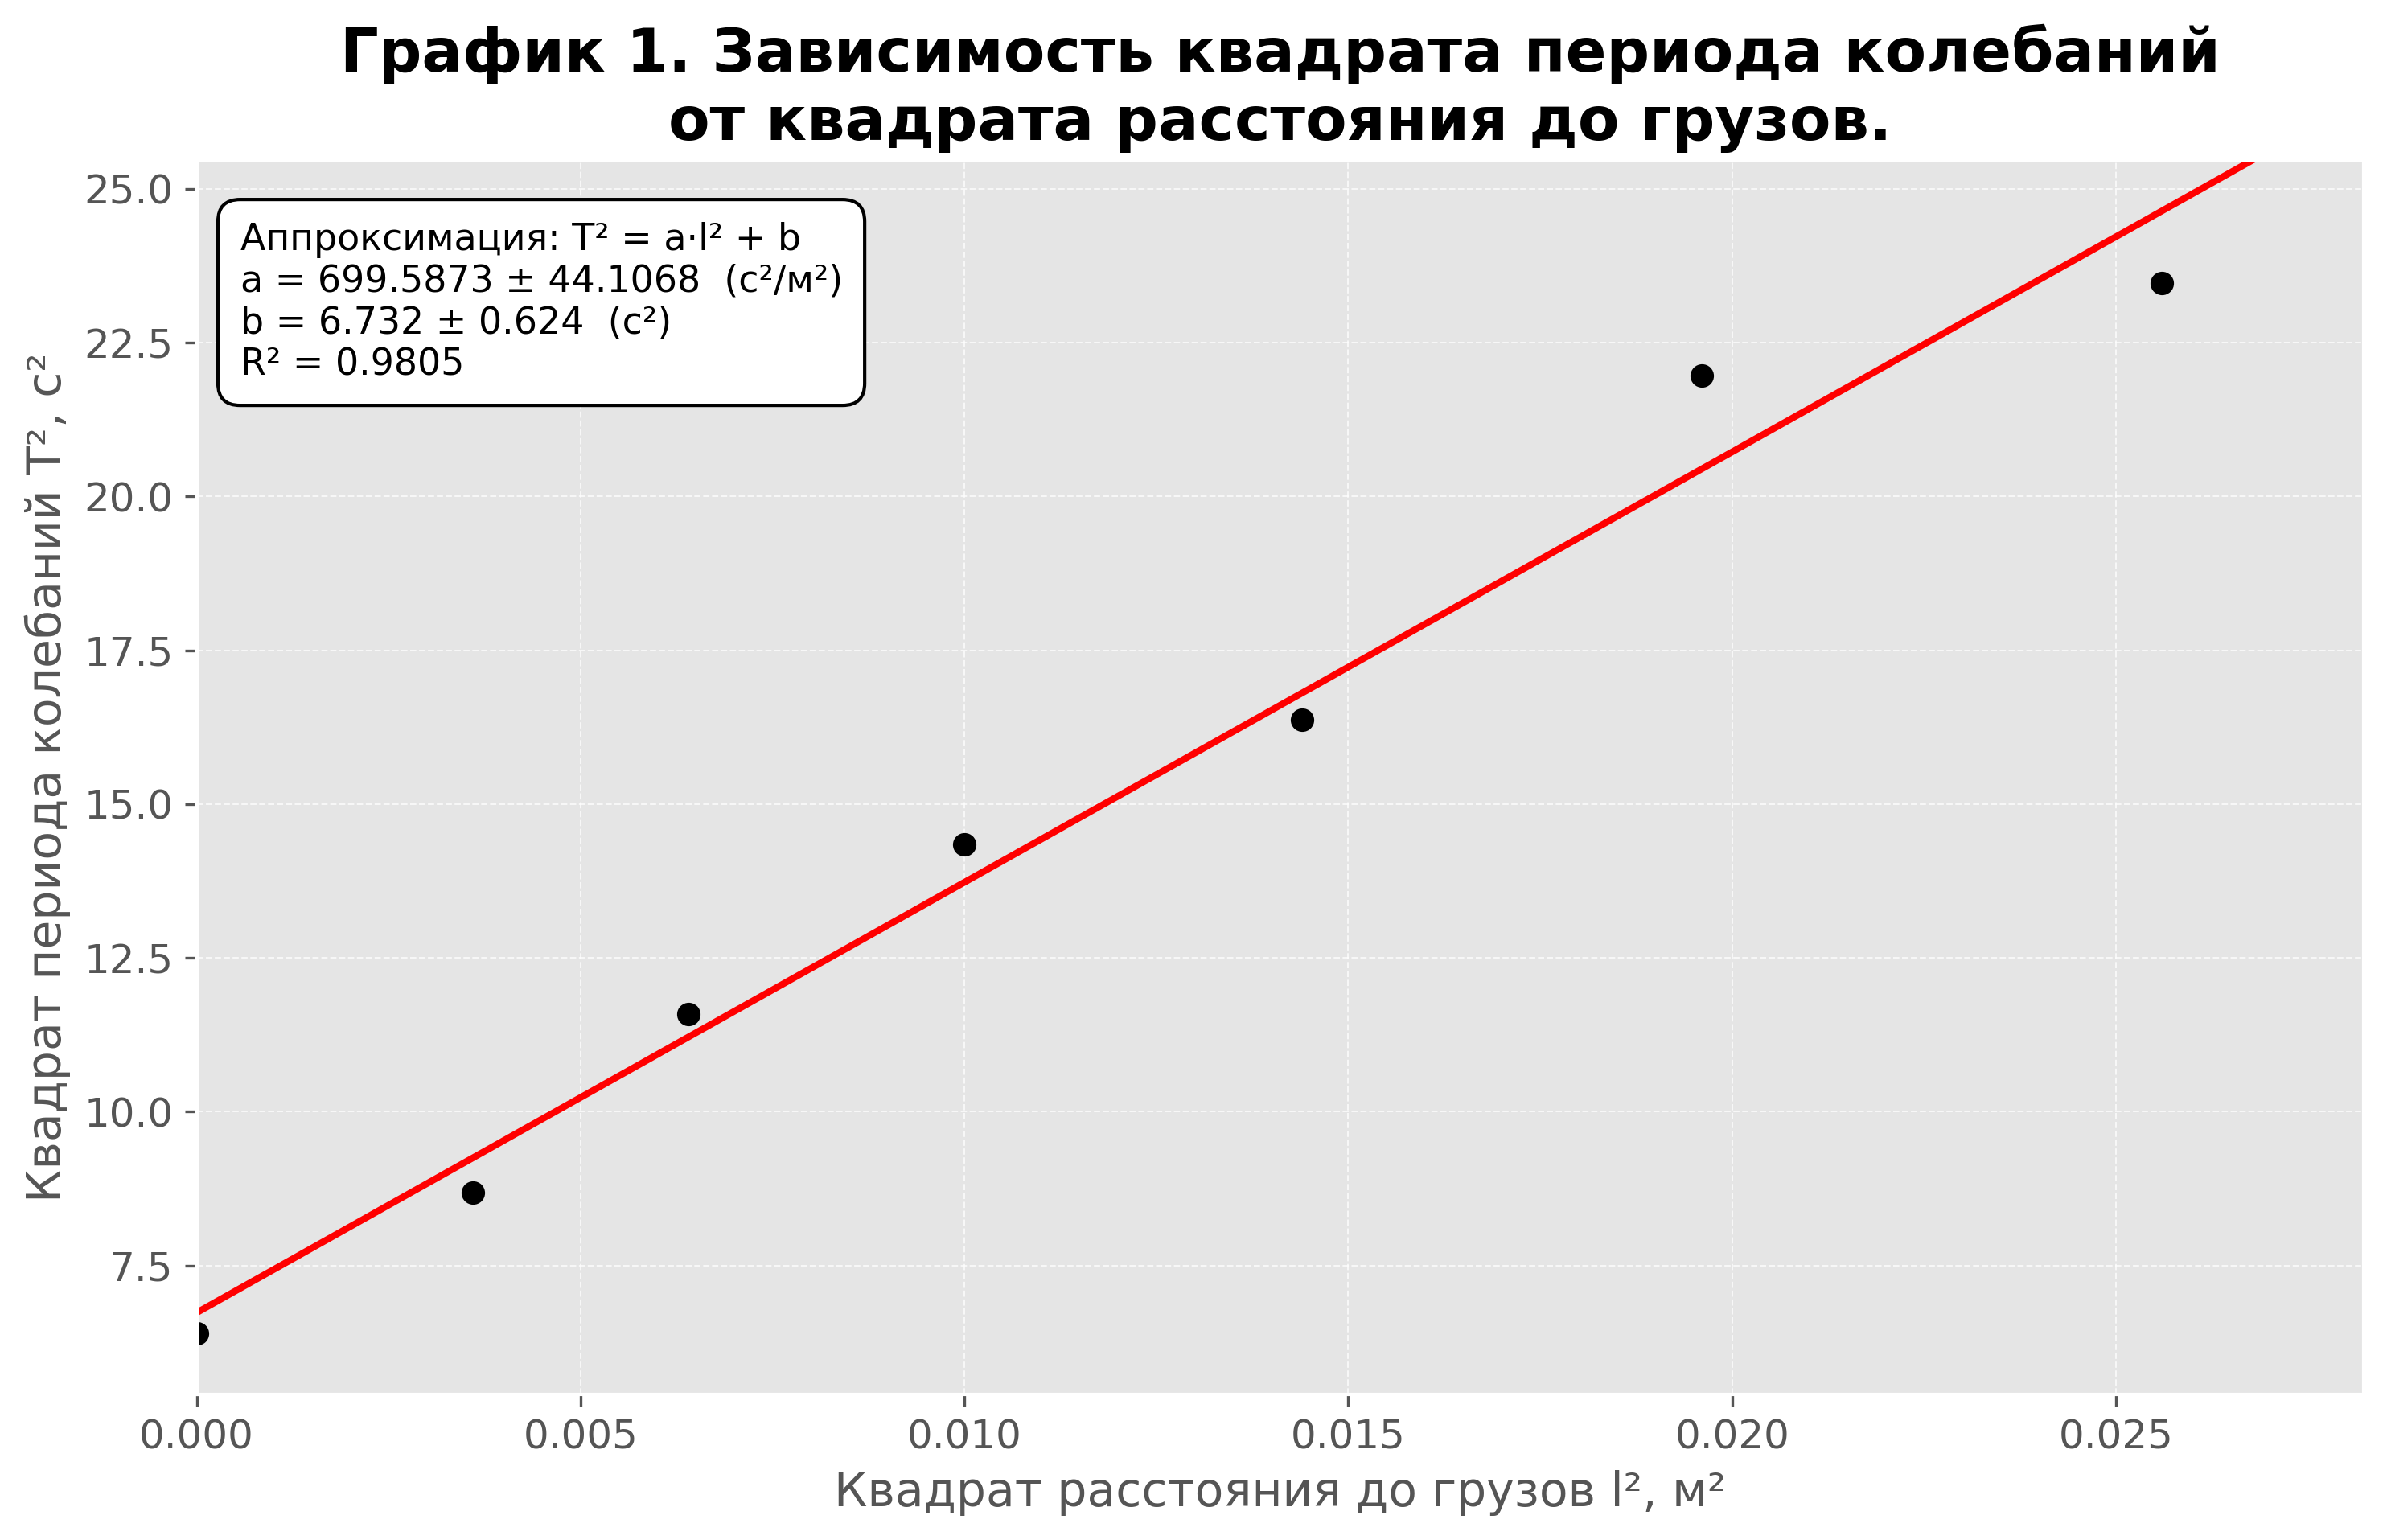
\includegraphics[width=0.8\linewidth]{picture1}
    \end{center}

    \begin{center}
        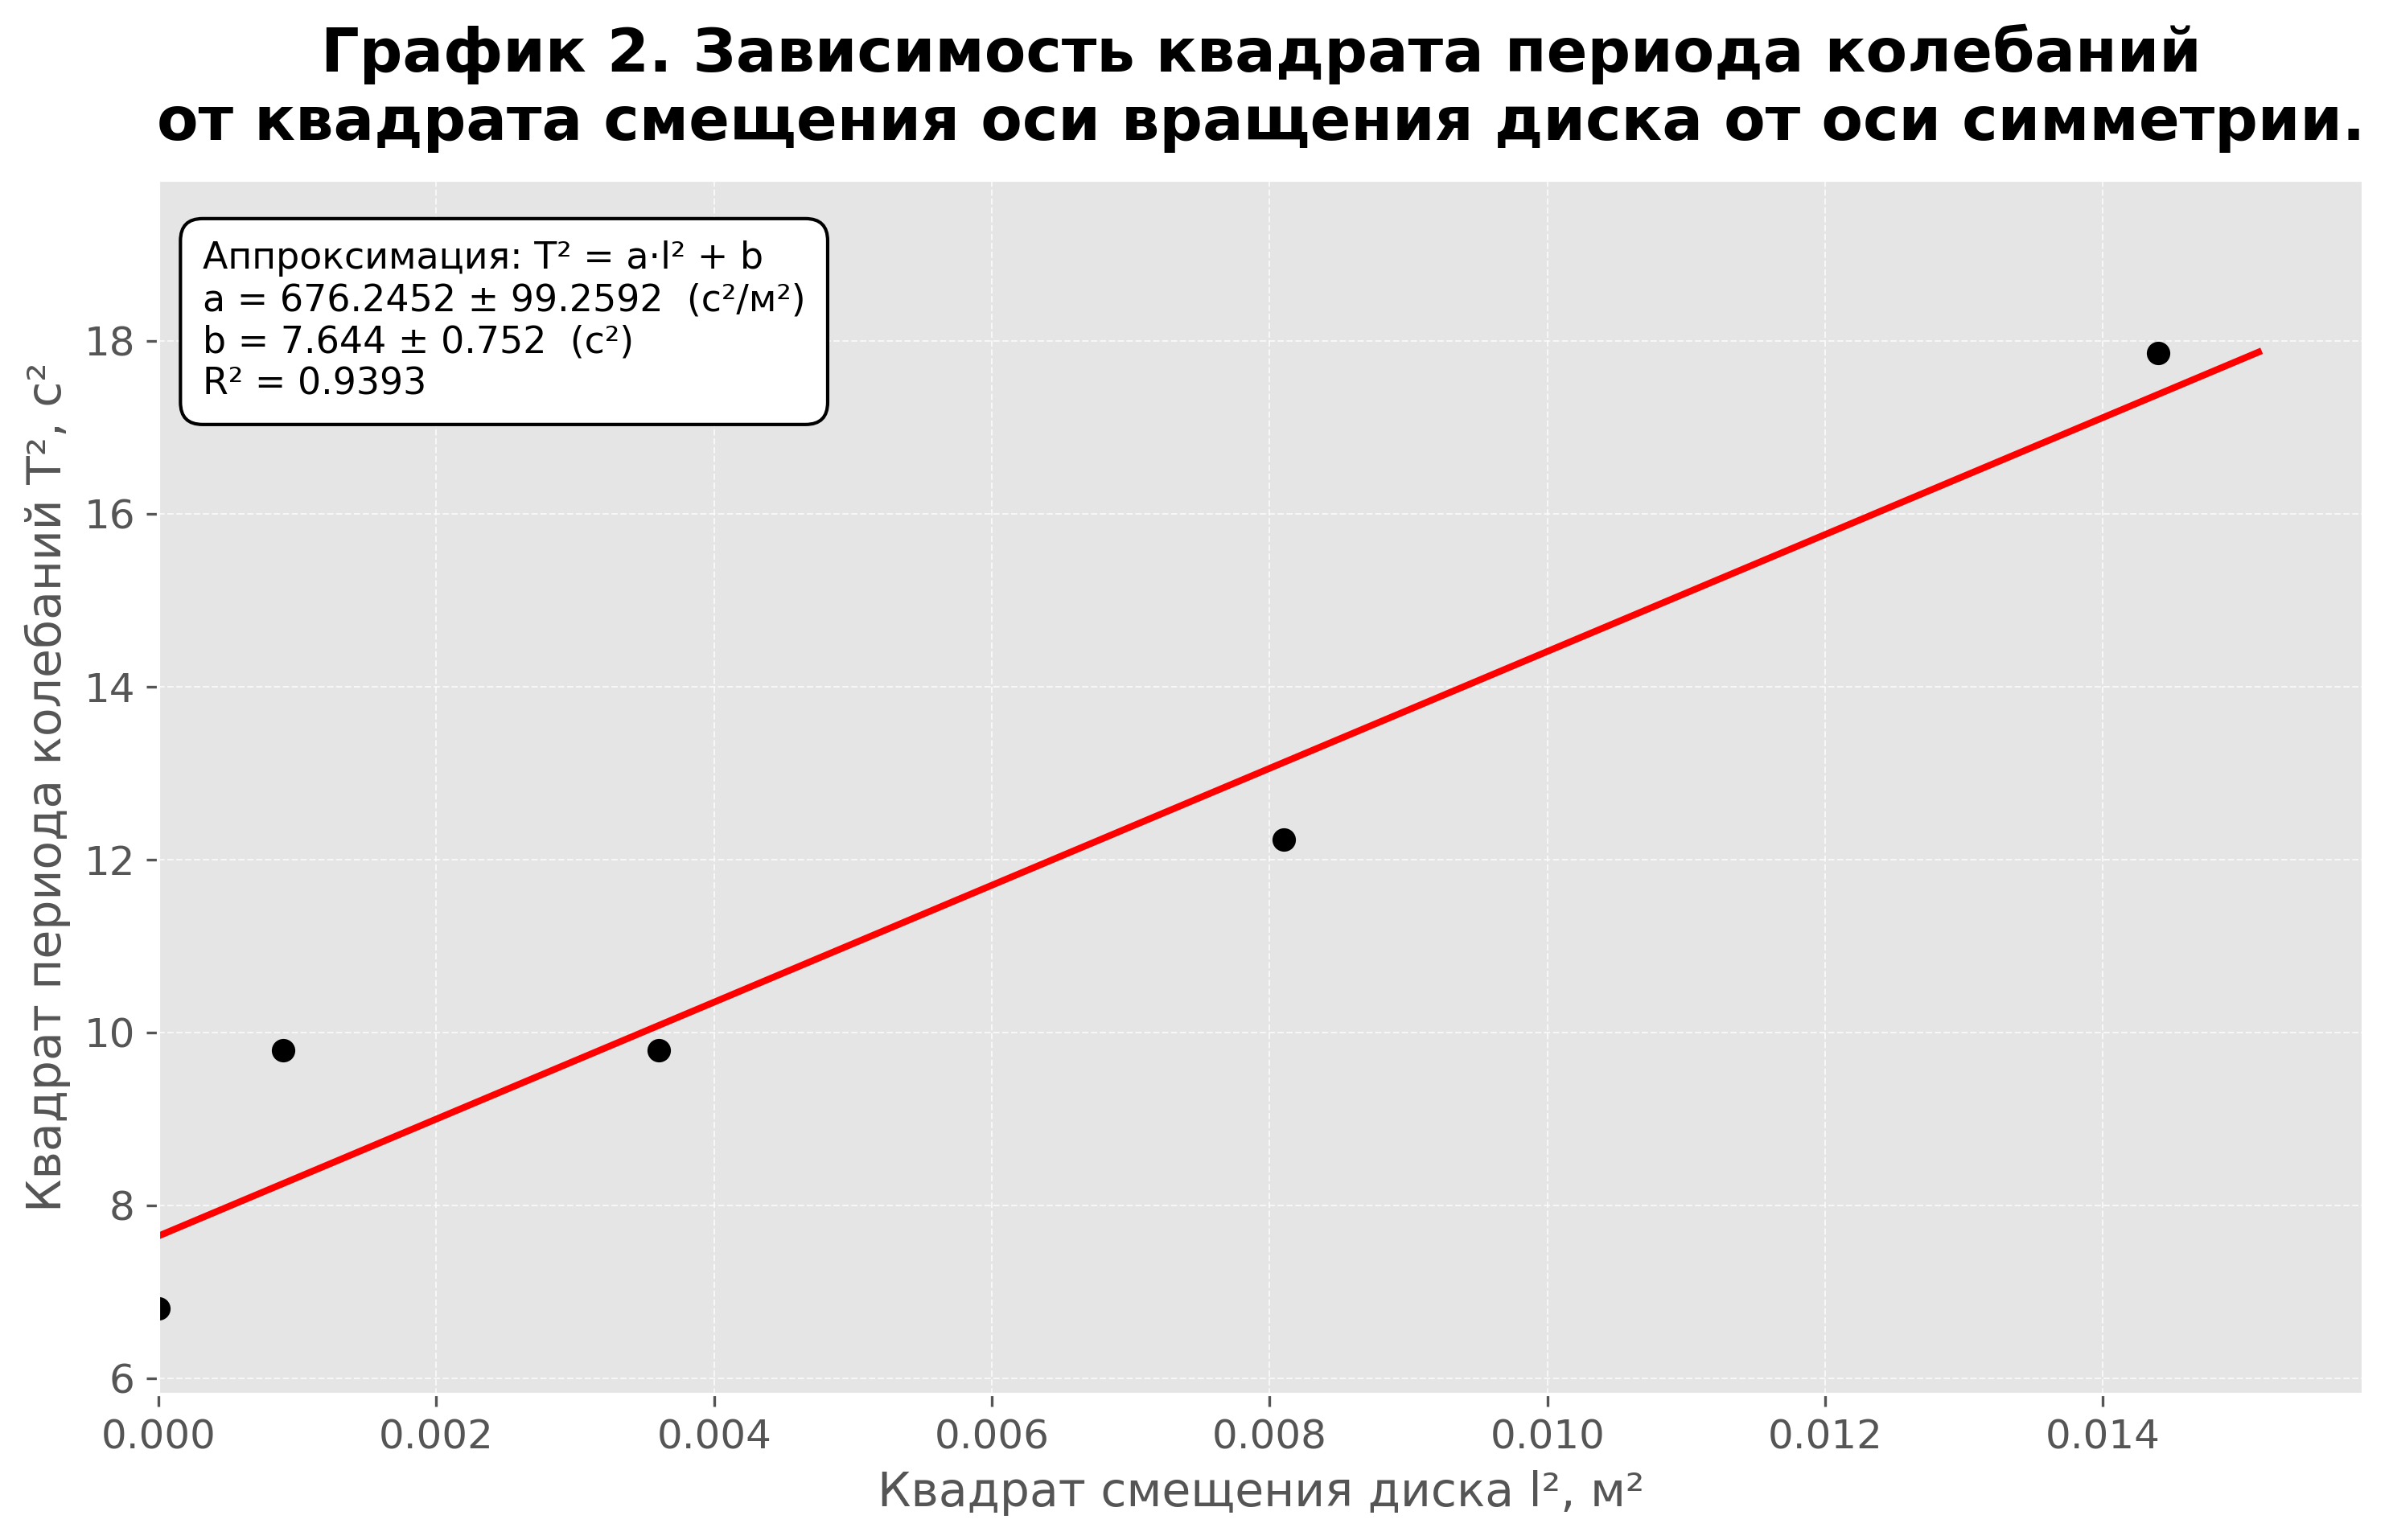
\includegraphics[width=0.8\linewidth]{picture2}
    \end{center}

    \section{Окончательные результаты}

    \begin{enumerate}
        \item Коэффициент угловой жесткости спиральной пружины.
        \[k = (21,4175 \pm 0,972)\cdot 10^{-3} \ \text{Н}\cdot\text{м}\]
        \item Центральный момент инерции штанги.
        \[I_{rod} = 3,47 \pm 0,673 \ \text{г}\cdot\text{м}^2\]
        \[I_{rod, \text{теор}} = 5,25504 \ \text{г}\cdot\text{м}^2\]
        \item Масса груза.
        \[m = 189.7675 \ \text{г}\]
        \[m_\text{факт} = 229 \ \text{г}\]
        \item Центральный момент инерции грузов.
        \[I_{c} = 0,091 \ \text{г}\cdot\text{м}^2\]
        \[I_{c, \text{теор}} = 0,134 \ \text{г}\cdot\text{м}^2\]
        \item Центральный момент инерции диска с отверстиями.
        \[I_{c} = 4.147 \ \text{г}\cdot\text{м}^2\]
        \[I_{c, \text{теор}} = 4,9618\ \text{г}\cdot\text{м}^2\]
        \item Центральный момент инерции шара.
        \[I_{c} = 1,598755 \pm 0,1872 \ \text{г}\cdot\text{м}^2\]
        \[I_{c, \text{теор}} = 1,95750 \ \text{г}\cdot\text{м}^2\]
        \item Центральный момент инерции сплошного диска.
        \[I_{c} = 1,354328 \pm 0,2407 \ \text{г}\cdot\text{м}^2\]
        \[I_{c, \text{теор}} = 1,70616 \ \text{г}\cdot\text{м}^2\]
        \item Центральный момент инерции полого цилиндра.
        \[I_{c} = 0,647190 \pm 0,1665 \ \text{г}\cdot\text{м}^2\]
        \[I_{c, \text{теор}} = 0,90750 \ \text{г}\cdot\text{м}^2\]
        \item Центральный момент инерции сплошного цилиндра.
        \[I_{c} = 0,4054 \pm 0,0817 \ \text{г}\cdot\text{м}^2\]
        \[I_{c, \text{теор}} = 0,57858 \ \text{г}\cdot\text{м}^2\]
    \end{enumerate}


    \section{Выводы и анализ результатов работы}

    ~


    В ходе работы были измерены периоды крутильных колебаний для различных твёрдых тел и на их основе найдены экспериментальные значения моментов инерции, которые затем были сопоставлены с теоретическими расчётами. Полученные значения моментов инерции в большинстве случаев заметно отличаются от теоретических (порядка 17\%), что указывает на наличие систематических погрешностей эксперимента.

    Графики зависимостей $T^2$ от смещения (или квадрата расстояния до оси) для систем «штанга с грузами» и «диск с отверстиями» в целом имеют близкий к линейному характер, что качественно подтверждает справедливость теоремы Гюйгенса–Штейнера в условиях данной установки. Основным источником расхождений можно считать недостаточно жёсткое и точное крепление тел на оси: из-за люфта и смещения положения равновесия фактический период колебаний уменьшался, что приводило к занижению экспериментально определённых моментов инерции по сравнению с теоретическими значениями.
    \section{Ответ по вопрос}

    Вопрос:

    В вашем эксперименте для первого положения груза (\(l_1 = 100\ \text{мм}\)) экспериментальная приведённая длина оказалась значительно больше теоретической: \(l_{\text{эксп}1} = (116{,}1 \pm 1{,}9)\ \text{мм}\) против \(l_{\text{теор}1} = 101{,}3\ \text{мм}\). При этом для двух других положений (\(l_2\) и \(l_3\)) расхождение составило менее \(3\ \%\). Вы предположили, что это ошибка при измерении, но какие конкретные систематические ошибки могли привести именно к увеличению эффективной приведённой длины для первого положения груза? Как вы думаете, могла ли ошибка быть связана с неправильной установкой угла наклона, неправильным позиционированием груза на стержне, или с чем-то другим?

    Ответ:

    Наиболее вероятная причина здесь - систематическая ошибка именно в геометрии первой установки: груз мог быть неправильно позиционирован на штанге (центр масс оказывался не на отметке \(100\ \text{мм}\) из‑за перекоса, люфта в креплении или неучтённого смещения от края до центра груза), а также возможно неправильное отсчитывание расстояния от оси. Такие ошибки как раз приводят к увеличению эффективного плеча и, следовательно, к увеличению экспериментальной приведённой длины только для первого положения, тогда как ошибка в установке угла отклонения, наоборот, для малых углов почти не влияет на период и вряд ли могла дать именно такое выборочное расхождение.


\end{document}